\documentclass{article}

%%%%%%%%%%%%%%%%%%%%%%%%%%%%%%%%
% PACKAGES
%%%%%%%%%%%%%%%%%%%%%%%%%%%%%%%%
\usepackage{times}
\usepackage{fullpage}
\usepackage{latexsym}
\usepackage{amsmath}
\usepackage{amssymb}
\usepackage{mathtools}
\usepackage{accents}
\usepackage{tikz}
\usepackage{pgfplots}
\usepackage[ruled]{algorithm}
\usepackage{algpseudocode}
\usepackage{dsfont}
\usepackage[bf]{caption}
\usepackage{hyperref}
\hypersetup{
    bookmarks=true,         % show bookmarks bar?
    unicode=false,          % non-Latin characters in AcrobatÕs bookmarks
    pdftoolbar=true,        % show AcrobatÕs toolbar?
    pdfmenubar=true,        % show AcrobatÕs menu?
    pdffitwindow=false,     % window fit to page when opened
    pdfstartview={FitH},    % fits the width of the page to the window
    pdftitle={My title},    % title
    pdfauthor={Author},     % author
    pdfsubject={Subject},   % subject of the document
    pdfcreator={Creator},   % creator of the document
    pdfproducer={Producer}, % producer of the document
    pdfkeywords={keyword1} {key2} {key3}, % list of keywords
    pdfnewwindow=true,      % links in new window
    colorlinks=true,       % false: boxed links; true: colored links
    linkcolor=red,          % color of internal links (change box color with linkbordercolor)
    citecolor=blue,        % color of links to bibliography
    filecolor=magenta,      % color of file links
    urlcolor=cyan           % color of external links
}
\usepackage{amsthm}
\usepackage{natbib}
\usepackage[capitalize]{cleveref}
\usepackage{graphicx}
\usepackage{parskip}
\usepackage{tikz} 
\usetikzlibrary{arrows,positioning} 
\pgfarrowsdeclarecombine{ring}{ring}{}{}{o}{o}
%\DeclareMathOperator{\ringarrow}{\raisebox{0.5ex}{\tikz[baseline]{\draw[ring->](0,0)--(2em,0);}}}
%%%%%%%%%%%%%%%%%%%%%%%%%%%%%%%%
% MACROS
%%%%%%%%%%%%%%%%%%%%%%%%%%%%%%%%
\newcommand{\defined}{\vcentcolon =}
\newcommand{\rdefined}{=\vcentcolon}
\newcommand{\E}[1]{\mathbb E\left[#1\right]}
\newcommand{\Var}{\operatorname{Var}}
\newcommand{\calF}{\mathcal F}
\newcommand{\sr}[1]{\stackrel{#1}}
\newcommand{\set}[1]{\left\{#1\right\}}
\newcommand{\ind}[1]{\mathds{1}\!\!\set{#1}}
\newcommand{\argmax}{\operatornamewithlimits{arg\,max}}
\newcommand{\argmin}{\operatornamewithlimits{arg\,min}}
\newcommand{\floor}[1]{\left \lfloor {#1} \right\rfloor}
\newcommand{\ceil}[1]{\left \lceil {#1} \right\rceil}
\newcommand{\eqn}[1]{\begin{align}#1\end{align}}
\newcommand{\eq}[1]{\begin{align*}#1\end{align*}}
\newcommand{\Ber}{\operatorname{Bernoulli}}
\renewcommand{\P}[1]{\operatorname{P}\left\{#1\right\}}
\newcommand{\N}[2]{\mathcal{N}\left({#1}\;,\;{#2}\right)}

\tikzset{
    %Define standard arrow tip
    >=stealth',
    %Define style for boxes
    observed/.style={
           circle,
           rounded corners,
           draw=black, thick,
           minimum width=2.5em,
           minimum height=2.5em,
           font=\footnotesize,
           text centered,
           scale=1,
           fill=blue!20!white},
     latent/.style={
           circle,
           rounded corners,
           draw=black, thick, dashed,
           minimum width=2.5em,
           minimum height=2.5em,
           font=\footnotesize,
           text centered,
           fill=black!10!white
           },
     empty/.style={
           circle,
           rounded corners,
           minimum width=.5em,
           minimum height=.5em,
           font=\footnotesize,
           text centered,
           },
    % Define arrow style
    pil/.style={
           o->,
           thick,
           shorten <=2pt,
           shorten >=2pt,},
    sh/.style={ shade, shading=axis, left color=red, right color=green,
    shading angle=45 }  
}


%%%%%%%%%%%%%%%%%%%%%%%%%%%%%%%%
% THEOREMS
%%%%%%%%%%%%%%%%%%%%%%%%%%%%%%%%
\theoremstyle{plain}
\newtheorem{theorem}{Theorem}
\newtheorem{proposition}[theorem]{Proposition}
\newtheorem{lemma}[theorem]{Lemma}
\newtheorem{corollary}[theorem]{Corollary}
\theoremstyle{definition}
\newtheorem{definition}[theorem]{Definition}
\newtheorem{assumption}[theorem]{Assumption}
\newtheorem{remark}[theorem]{Remark}
\newtheorem{example}[theorem]{Example}

\title{Partial Identifiability}


\begin{document}
\def\ci{\perp\!\!\!\perp}


\begin{figure}[H]
	\centering    
          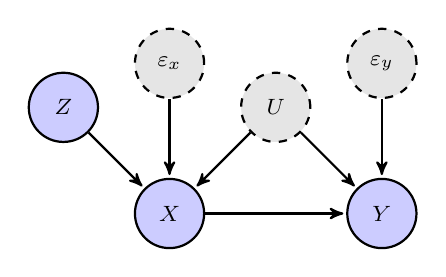
\begin{tikzpicture}[->,>=stealth',shorten >=1pt,auto,node distance=1cm,
  thick,main node/.style={observed}, hidden/.style={empty},background rectangle/.style={fill=olive!45}]
 %nodes
\node[main node](1){$Z$};
\node[main node, below right=of 1](2){$X$};
\node[latent, above right=of 2](3){$U$};
\node[main node, below right=of 3](4){$Y$};
\node[latent, above=of 2](5){$\varepsilon_x$};
\node[latent, above=of 4](6){$\varepsilon_y$};
 \path[every node/.style={font=\tiny}]
    (1) edge (2)
    (3) edge (2) edge (4)
    (2) edge (4)
    (5) edge (2)
    (6) edge (4);
\end{tikzpicture}
\end{figure}

\eq{
Z \sim \N{\mu_z}{v_z}\\
U \sim \N{\mu_u}{v_u}\\
\varepsilon_x \sim \N{0}{\epsilon_x}\\
\varepsilon_y \sim \N{0}{\epsilon_y}}
\eq{
X &=  w_{x0} + w_{xz}Z + w_{xu}U + \varepsilon_x \\
Y &= w_{y0}+w_{yu}U+w_{yx}X+\varepsilon_y
}

As all the exogenous variables ($Z,U,\varepsilon_x, \varepsilon_y$) are Gaussian and all the functions linear, $\P{Z,U,X,Y}$ and thus  $\P{Z,X,Y}$ is a multivarite Gaussian.

\eq{
\P{Z,X,Y} \sim \N{\begin{bmatrix}
\mu_z\\
w_{x0}+w_{xz} \mu_z+w_{xu}\mu_u\\
(w_{y0}+w_{yx} w_{x0})+(w_{yu}+w_{yx}w_{xu})\mu_u + w_{yx}w_{xz}\mu_z
\end{bmatrix}}
{\Sigma}
}

where,

\eq{
\Sigma = \begin{bmatrix}
\Sigma_{zz} & \Sigma_{zx} & \Sigma_{zy} \\
. & \Sigma_{xx} & \Sigma_{xy} \\
. & . & \Sigma_{yy}
\end{bmatrix} = \begin{bmatrix}
v_z & w_{xz}\Sigma_{zz} & w_{yx}\Sigma_{zx} \\
. & w_{xz}^2 v_z+w_{xu}^2 v_u +\epsilon_x & w_{xu}w_{yu}v_u +w_{yx}\Sigma_{xx} \\
. & . &w_{yx}^2\Sigma_{xx} +2w_{yx}w_{yu}w_{xu}v_u +w_{yu}^2 v_u+\epsilon_y
\end{bmatrix}
}

We want to identify,

\eq{
Y|do(X=x) &= w_{y0}+w_{yu}U+w_{yx}x+\varepsilon_y  \\
\implies \P{Y|do(X=x)} &=\N{w_{y0}+w_{yu}\mu_u+w_{yx}x}{w_{yu}^2 v_u+\epsilon_y}\\
&=\N{\mu_y+w_{yx}(x-\mu_x)}{w_{yu}^2 v_u+\epsilon_y}\\
&= \N{\mu_y+ \frac{\Sigma_{zy}}{\Sigma_{zx}}(x-\mu_x)}{\Sigma_{yy} + \frac{\Sigma_{zy}}{\Sigma_{zx}}\left(\frac{\Sigma_{zy}}{\Sigma_{zx}}\Sigma_{xx} - 2\Sigma_{xy} \right)}
}

The final equation is purely in terms of $x$ and properties of the joint (non interventional) distribution $\P{X,Y,Z}$ so we get unbiased point estimates for both the mean and variance of $\P{Y|do(X=x)}$ provided $\Sigma_{zx} \neq 0$, that is if $v_z \neq 0$ and $w_{xz} \neq 0$. 

We can identify the difference in the average causal effect for two interventions on $X$ (assuming $v_z,w_{xz} > 0$) .
\eq{
\E{Y|do(X=x)} - \E{Y|do(X=x')} = w_{yx}(x-x') = \frac{\Sigma_{zy}}{\Sigma_{zx}}(x-x')
}

We can also identify the variance of $\P{Y|do(X=x)}$.

\eq{
w_{yu}^2 v_u+\epsilon_y = \Sigma_{yy} + \frac{\Sigma_{zy}}{\Sigma_{zx}}\left(\frac{\Sigma_{zy}}{\Sigma_{zx}}\Sigma_{xx} - 2\Sigma_{xy} \right)
}

Conditional distributions are also gaussian.

\eq{
%P(Y|X=x)& \sim \N{\mu_y + \Sigma_{yx}\Sigma_{yy}^{-1}(x-\mu_x)}{\Sigma_{yy} - \Sigma_{yx}\Sigma_{yy}^{-1}\Sigma_{yx}^T}\\
P(Y|X=x) &= \N{\mu_y+\frac{\Sigma_{xy}}{\Sigma_{yy}}(x-\mu_x)}{\Sigma_{yy} - \frac{\Sigma_{xy}^2}{\Sigma_{yy}}} \\
 &= 
}

Intuitively we want the link $Z \rightarrow X \rightarrow Y$ to be stronger than $Z \rightarrow X\rightarrow U \rightarrow Y$. If we can see that X is mostly determined by Z then this must be the case. Similarly it would be good if Y is strongly determined by X (then U cannot have much influence). Quantify this statement.

Start by looking at the variance of $P(X|Z)$ - relative to the mean?
Also the variance of $P(Y|X)$. 

Look at some extreme examples - what happens when $Z$ exactly determines $X$. 

We know all the diagonal terms in the covariance matrix are positive. This will create bounds on terms that cannot be exactly identified.



\end{document}

